\documentclass[10pt,a4paper,twocolumn,twoside]{article}
\usepackage[utf8]{inputenc}
\usepackage[catalan]{babel}
\usepackage{multicol}
\usepackage{graphicx}
\usepackage{fancyhdr}
\usepackage{times}
\usepackage{titlesec}
\usepackage{multirow}
\usepackage{lettrine}
\usepackage[top=2cm, bottom=1.5cm, left=2cm, right=2cm]{geometry}
\usepackage[figurename=Fig.,tablename=TAULA]{caption}
\usepackage{hyperref}
\usepackage{listings}

\lstset{
  breaklines=true,
  tabsize=2,
}

\captionsetup[table]{textfont=sc}

\titlespacing*{\section}{0pt}{0.5cm}{0.2cm}
\titlespacing*{\subsection}{0pt}{0.5cm}{0.2cm}


\graphicspath{{img/}}

\author{\normalsize\sffamily Kevin Martín Fernández}
\title{\huge{\sffamily GEOSpectralSimulator}}
\date{}

\newcommand\blfootnote[1]{%
  \begingroup
  \renewcommand\thefootnote{}\footnote{#1}%
  \addtocounter{footnote}{-1}%
  \endgroup
}

%No ident
\setlength\parindent{0pt}

%
%\large\bfseries\sffamily
\titleformat{\section}
{\large\sffamily\scshape\bfseries}
{\textbf{\thesection}}{1em}{}

%List counter enumerate
\renewcommand{\labelenumii}{\theenumii}
\renewcommand{\theenumii}{\theenumi.\arabic{enumii}.}
\renewcommand{\labelenumiii}{\theenumiii}
\renewcommand{\theenumiii}{\theenumii \arabic{enumiii}.}

\begin{document}

\fancyhead[LO]{\scriptsize Kevin Martín: GEOSpectralSimulator GEOSS}
\fancyhead[RO]{\thepage}
\fancyhead[LE]{\thepage}
\fancyhead[RE]{\scriptsize EE/UAB TFG INFORMÀTICA: GEOSpectralSimulator}

\fancyfoot[CO,CE]{}

\fancypagestyle{primerapagina}
{
   \fancyhf{}
   \fancyhead[L]{\scriptsize TFG EN ENGINYERIA INFORMÀTICA, ESCOLA D'ENGINYERIA (EE), UNIVERSITAT AUTÒNOMA DE BARCELONA (UAB)}
   \fancyfoot[C]{\scriptsize June 2019. Escola d'Enginyeria (UAB)}
}

%\lhead{\thepage}
%\chead{}
%\rhead{\tiny EE/UAB TFG INFORMÀTICA: TÍTOL (ABREUJAT SI ÉS MOLT LLARG)}
%\lhead{ EE/UAB \thepage}
%\lfoot{}
%\cfoot{\tiny{February 2015, Escola d'Enginyeria (UAB)}}
%\rfoot{}
\renewcommand{\headrulewidth}{0pt}
\renewcommand{\footrulewidth}{0pt}
\pagestyle{fancy}

%\thispagestyle{myheadings}
\twocolumn[\begin{@twocolumnfalse}

{
\vspace*{-1cm}
\maketitle
}

\thispagestyle{primerapagina}
%\twocolumn[\begin{@twocolumnfalse}
%\maketitle
%\begin{abstract}
\begin{center}
\parbox{0.915\textwidth}
{\sffamily\small
\textbf{Abstract--} Resum
\\
\\
\textbf{Keywords-- }
Simulator, Terrain, Satelite, Multiespectre, Unreal Engine\\
\\
%\end{abstract}
}

\bigskip

{\vrule depth 0pt height 0.5pt width 4cm\hspace{7.5pt}%
\raisebox{-3.5pt}{\fontfamily{pzd}\fontencoding{U}\fontseries{m}\fontshape{n}\fontsize{11}{12}\selectfont\char70}%
\hspace{7.5pt}\vrule depth 0pt height 0.5pt width 4cm\relax}

\end{center}

\bigskip
%\end{abstract}
\end{@twocolumnfalse}]

\blfootnote{$\bullet$ E-mail de contacte: kevinmf94@gmail.com}
\blfootnote{$\bullet$ Menció realitzada: Enginyeria de Computació}
\blfootnote{$\bullet$ Treball tutoritzat per: Felipe Lumbreras Ruíz}
\blfootnote{$\bullet$ Curs 2018/19}

\vspace{-1cm}
\section{Introduction}
The simulation of the real world for the generation of synthetic images is a scope in which you are looking to represent the real world more accurately possible, in this way can generate synthetic information that represents real environments that can represent a danger (for the natural environment, people, etc) or a high economic cost.
\\
\\
On this project you want to get that is able to by means of elevation maps and aerial images of real terrains generates a simulated environment that it can generate its image datasets, which can be used in multiple areas of the computation learning. Also, it can simulate flying, see a geographical area or expand this project in other environments that uses a geographic information. That geographical information it can provided from multiple sources this allows to work with a lot of external data.

\section{Objectius}

En aquest apartat determinarem els diferents objectius del projecte en format de jerarquia per tal de veure la dependència entre els diferents objectius:

\begin{enumerate}
  \item Analitzar
  
  \item Definir
  \begin{enumerate}
    \item Definir mòduls pel projecte
    \item Definir l'estructura del software
    
    \item Definir plataformes utilitzades
    \begin{enumerate}
    	\item Definir els mòduls a desenvolupar
	    \item Definir la comunicació entre els mòduls
    	\item Definir estructura de les dades que rebrà Unreal Engine
  	\end{enumerate}
  \end{enumerate}
  
  \item Desenvolupar
  \begin{enumerate}
    \item Desenvolupar mòdul de transformació i obtenció de dades
    \item Desenvolupar mòdul gràfic (Ureal Engine)
    \begin{enumerate}
    	\item Desenvolupar la interfície del menú
	    \item Desenvolupar la lògica del vehicle
    	\item Desenvolupar codi per la carrega de terreny y material
    	\item Desenvolupar llibreria RPC per el control del entorn
  	\end{enumerate}
  	
  	\item Desenvolupar mòdul de scripting
  	\begin{enumerate}
    	\item Desenvolupament client que controlarà el vehicle
  	\end{enumerate}
  	
  	\item Integrar els mòduls d'AirSim en Unreal Engine
  	\begin{enumerate}
    	\item Integrar mòdul de Segmentació en el projecte
  	\end{enumerate}
  	
  	\item Desenvolupar altres capes d'informació
  \end{enumerate}
  
  \item Testejar
  \begin{enumerate}
    \item Fer provés del mòdul de transformació de dades
    \item Fer provés del mòdul gràfic
    \item Fer provés del mòdul de control per scripting
    \begin{enumerate}
    	\item Elaborar script d'exemple
	    \item Provar script d'exemple
  	\end{enumerate}
  \end{enumerate}
  
  \item Documentar
  \begin{enumerate}
    \item Redactar informe inicial
    \item Redactar informe de seguiment I
    \item Redactar informe de seguiment II
    \item Redactar l'informe final
    \item Elaborar proposta de presentació
    \item Elaborar pòster
    \item Gestionar la documentació del dossier
  \end{enumerate}
  
\end{enumerate}

\section{Methodology}
In this project its decide uses a methodology of Agile\cite{agile} style, this allows to identify more efficiently the little parts that compose the project, besides adapt to the changes. More concretely has used a technique called Kanban\cite{kanban} which consists in organizing this backlog (tasks of short duration) on cards that will be placed on a board according to the point of the life cycle on the tasks founds it. For this to be used the Trello\cite{trello} software that can see the boards on web browser, create cards and move it between different lists.

\subsection{Gant Diagram}

In order to manage a project you must also include a Gant diagram done with excel. In this diagram several tasks and subtasks are contemplated in order to make a prediction of the work done, the approximate time is what it will take for each task, this will allow an approximation of the time that the project behaves in this way.

\section{State of the art}
\label{estatart}

Currently exists diverse applications for the generation of images in simulated environments with the finality of generating data used in machine learning algorithms.

In this scope one of the most import is AirSim\cite{airsim} developed by Microsoft and Carla SIMULATOR\cite{carla} developed by ''Centre de Visio per Computador (CVC)'', also it's analyse others, how can they be LESS\cite{less}, DIRSIG {dirsig} or Google Earth Engine\cite{googleearth} of more specific scope.

\subsection{AirSim}
AirSim is a graphic simulator made with Unreal Engine, this simulator has the purpose of generating synthetic images on fake environments, it incorporates multiple modules that are offered the next functionalities (You can see an example in the figure \ref{fig-airsim}):

\begin{itemize}
  \item Simulation of cars.
  \item Simulation of drones.
  \item Compatibility with real drone controllers.
  \item Recording.
  \item Depth view.
  \item Segmentation view.
  \item Rain effects.
  \item Control of illumination according to the daily hours.
  \item Control of vehicles through a python script.
\end{itemize}

\begin{figure}[!h]
\centering
  	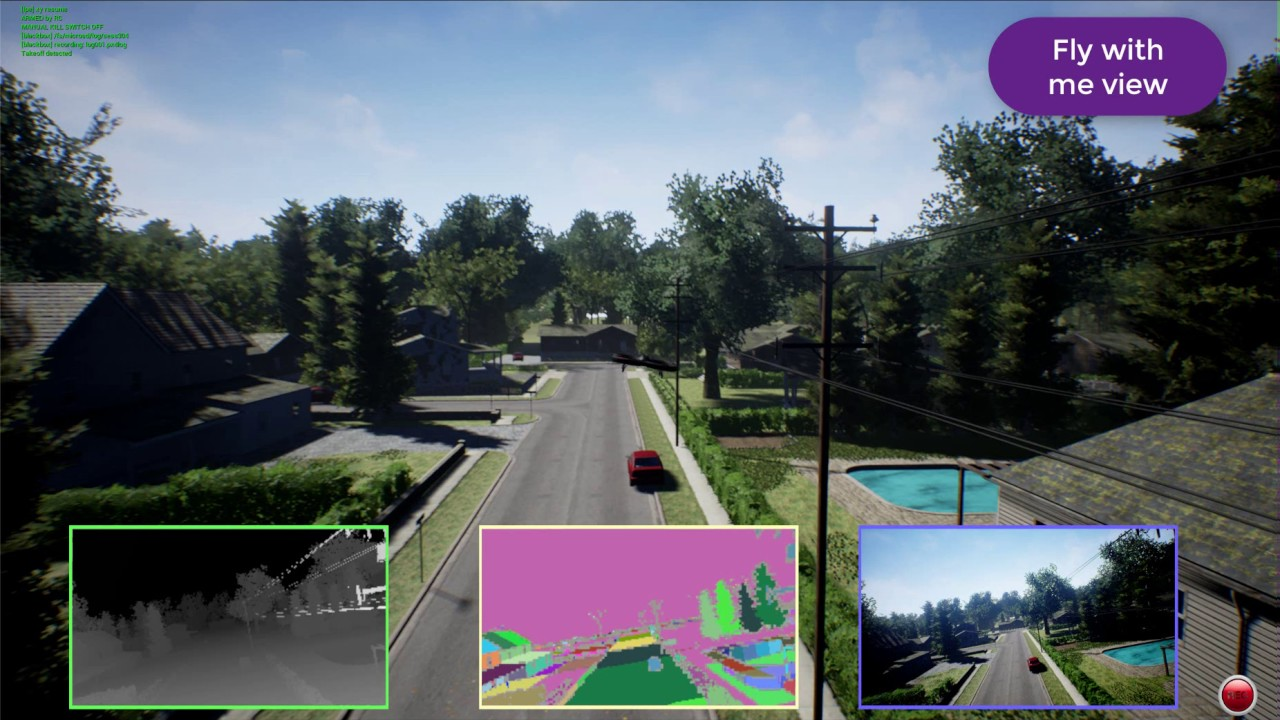
\includegraphics[width=0.4\textwidth]{airsim}
	\caption{AirSim simulator}
	\label{fig-airsim}
\end{figure}

\subsection{Carla SIMULATOR}
The Carla is a graphical simulator made on the Unreal Engine, this simulator has the finality of generating images on a fake environment with the maximum realism so that possible to generate images that they can serve to a made learning the neural networks able to drive safely a autonomous car taking into the unlikely cases that are difficult to generate in the real world. Its environment has the next functionalities:

\begin{itemize}
  \item Simulation of cars.
  \item Depth view.
  \item Segmentation view.
  \item Simulation of traffic, pedestrians, etc.
  \item Control of the actors (traffic, pedestrian, cameras, etc) with a python script.
\end{itemize}

\subsection{LESS}
LESS is a model of the radiation (You can see an example, in the figure \ref{fig-lessradiacio}) generated on a three-dimensional object/terrain for different rays, generating from a technique of ray-tracing its able to simulate data and images over realistic three-dimensional scenes. This model implements a method of follow weighted photons for simulating the effect of multi-spectral bidirectional reflectance.

\begin{figure}[!h]
\centering
  	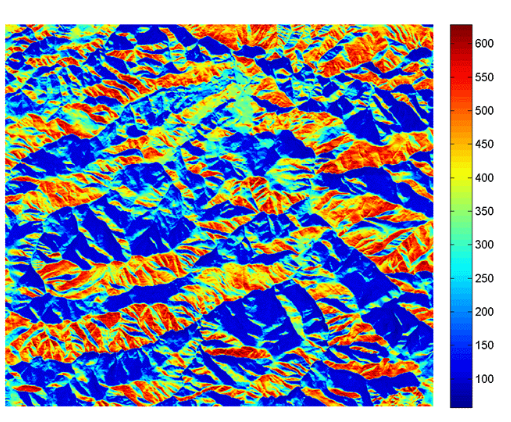
\includegraphics[width=0.4\textwidth]{lessradiacio}
	\caption{Example of results of the radiation of a terrain}
	\label{fig-lessradiacio}
\end{figure}

\subsection{DIRSIG}
The model of Digital Imaging and Remote Sensing Image Generation (DIRSIG) is a model of generation of synthetic images developed by the lab of Digital Imaging and Remote Sensing of the Rochester Institute of Technology. The model can produce one band images, multispectral or hiperspectral from visible trough of the infrared thermal region of the electromagnetic spectral. You can see an example generated by DIRSIG on the figure \ref{fig-tacoma}.

\begin{figure}[!h]
\centering
  	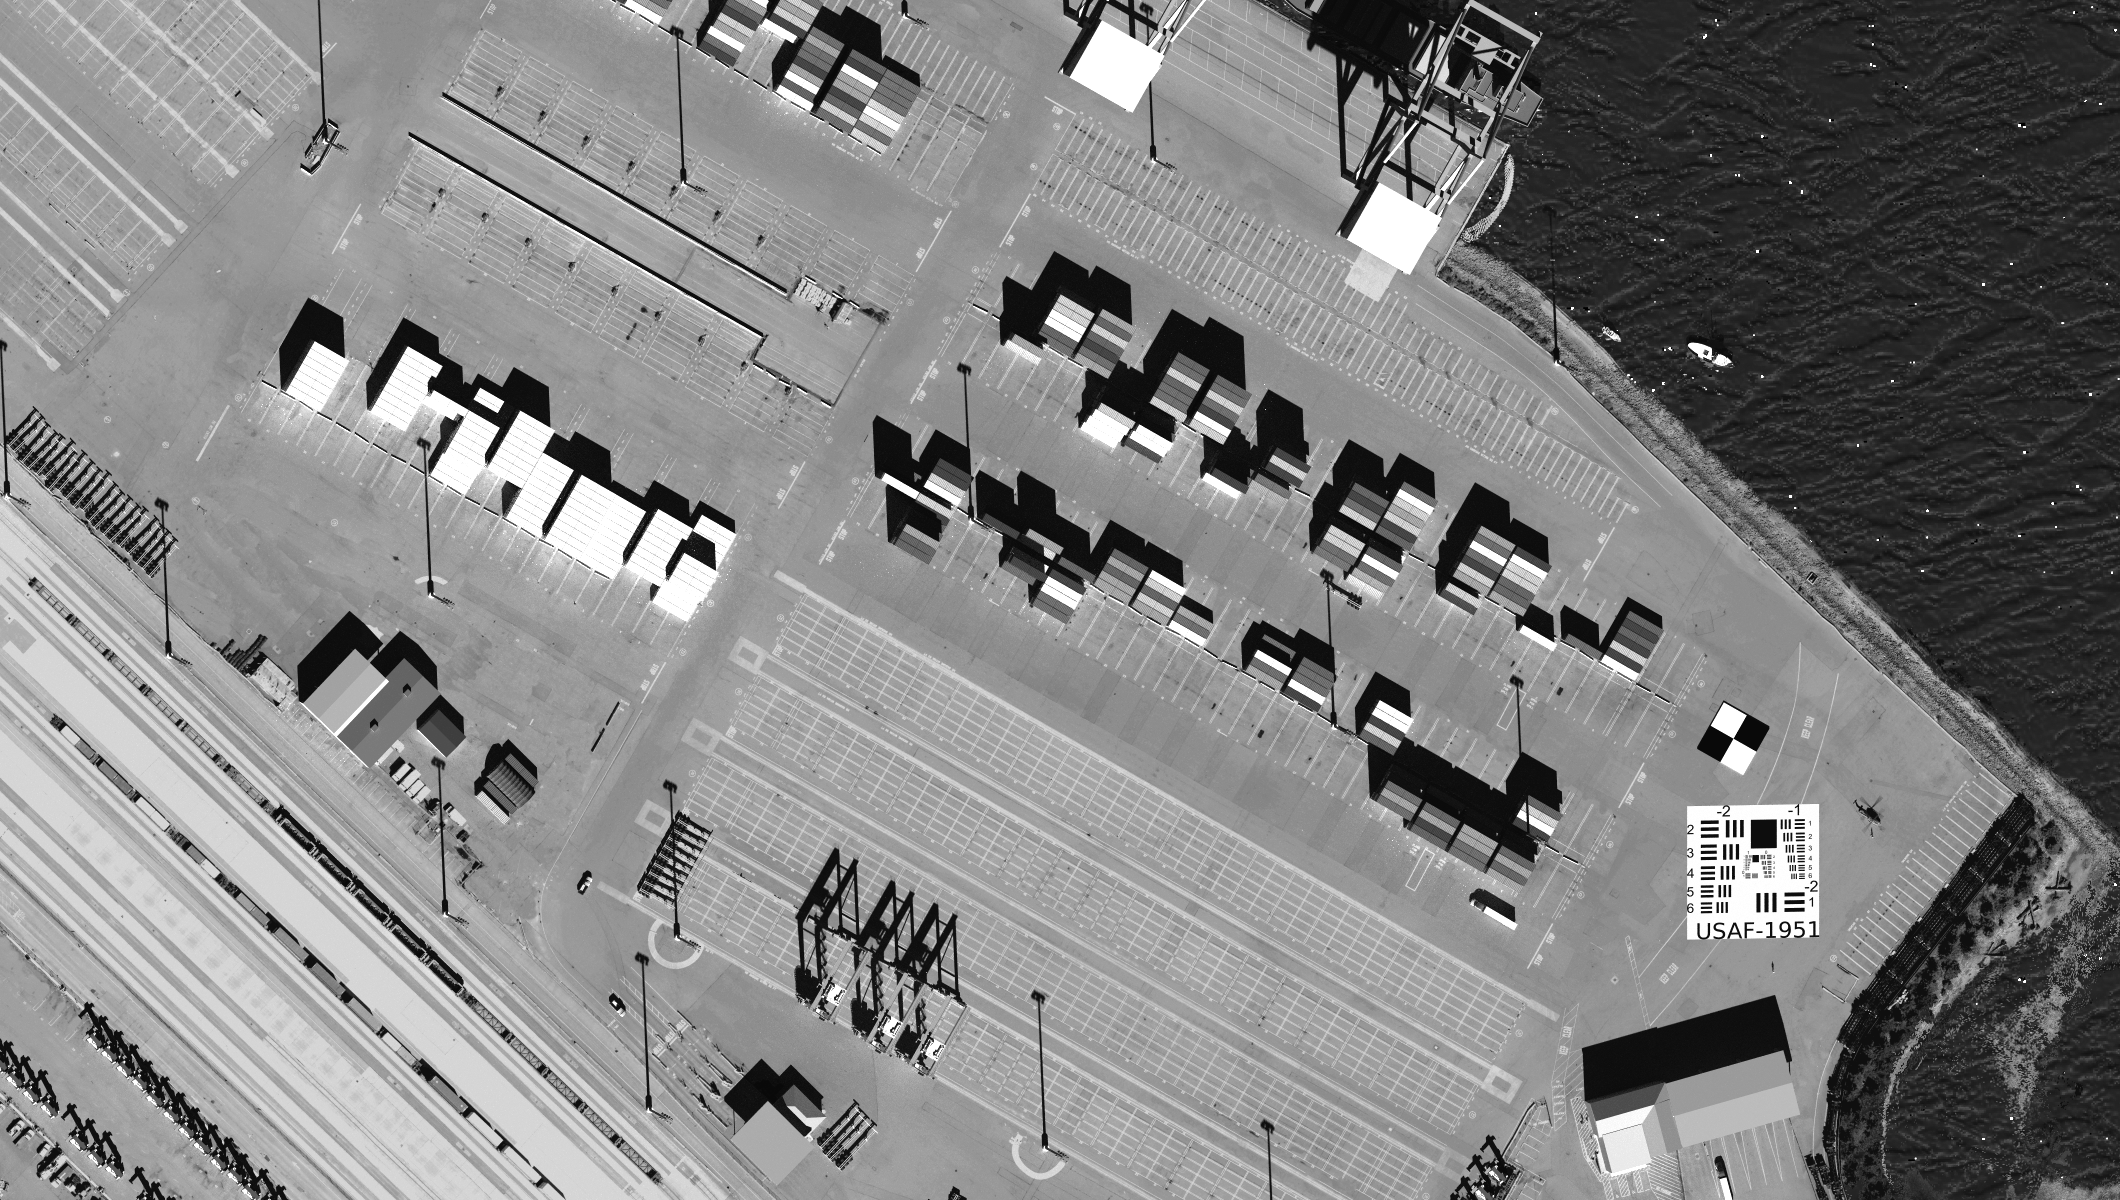
\includegraphics[width=0.4\textwidth]{tacoma}
	\caption{Frame from the Tacoma port}
	\label{fig-tacoma}
\end{figure}

\subsection{Google Earth Engine}

Google Earth Engine is a project by Google, dedicated to offer the necessary tools to be able to analyse and visualize geospacial data, intended for an academy studies, non-profit institutions, companies and governments. The principal features of the Google Earth Engine are:

\begin{itemize}
  \item We can work with datasets from different satellites such as LANDSAT, MODIS, SENTINEL, etc.
  \item Incorporate a work environment to manipulate the data and wide API that allows us to combine images from different spectral, see it on a world map, export data to Google Drive and more.
\end{itemize}

\section{Structure of project}
In order to determine the project structure, it's study the diverse alternatives viewed on section \ref{estatart}. Will be analysed the structure from AirSim and Carla with the objective of deciding the ownership structure and the external libraries to incorporate them into the project.

\subsection{AirSim} 
AirSim is composed of multiple modules written in various languages, as can be seen below:

\begin{itemize}
	\item \textbf{AirLib (C++)}: Module for Unreal Engine that provides the base classes to communicate through the RPC protocol and control the simulated vehicles.
	\item \textbf{DroneServer (C++)}: Server to receive orders from RPC client.
  	\item \textbf{DroneShell (C++)}: Shell client to send orders to the Server.
  	\item \textbf{PythonClient (Python)}: Client to send orders trough RPC, also includes code to the manipulation of images.
  	\item \textbf{SGM (C++)}: Code to manipulate images and generate the segmentation view.
    \item \textbf{Unity (C\# i C++)}: Unity version, includes a modules to see the AirSim information.
    \item \textbf{Unreal Engine (C++)}: Unreal version, includes a modules to see the AirSim information.
\end{itemize}

\subsection{Carla SIMULATOR}

Carla SIMULATOR is composed for multiple modules as you can see in the figure \ref{fig-carlamodules} written in multiple languages. The modules of Carla are:

\begin{figure}[!h]
\centering
  	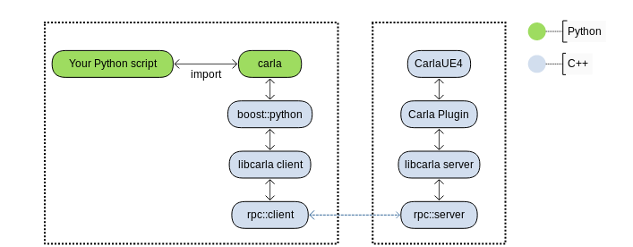
\includegraphics[width=0.5\textwidth]{carlamodules}
	\caption{Relation between the modules of Carla}
	\label{fig-carlamodules}
\end{figure}

\begin{itemize}
 \item \textbf{LibCarla (C++)}: The main library of Carla, is in charge of the logic of the simulation.
 \item \textbf{Unreal (C++)}: Graphic engine with the Carla plug-in, this includes all the functionalities added to Unreal.
 \item \textbf{PythonAPI (Python)}: The API allows sending orders to the Carla module that works like server, this API it's useful to make own scripts.
\end{itemize}


\subsection{The structure chosen}

Analysing multiple projects with similar features, it's decide for a own structure as we can see in the figure \ref{fig-dronsimulatormodules} being able to use something modules with other open-source projects. Its make this decision due to the fact that the other projects are based on the creation of terrain predefined on Unreal Editor, the opposite to the finality of this project in which its make terrain automatically provided by real data.

\begin{figure}[!h]
\centering
  	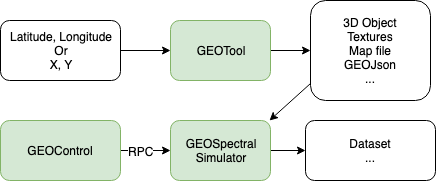
\includegraphics[width=0.45\textwidth]{structuretfg}
	\caption{Structure of GEOSpectralSimulator}
	\label{fig-dronsimulatormodules}
\end{figure}

Our project will consist of these modules:

\begin{itemize}
  \item \textbf{GEOTool (Python)}: This module has the finality of provides the needed tools for obtaining and adapt the data from some standards for geographical data web-service with the objective of can import this data on any graphic motor, it can generate diverse layers of data for the downloaded terrains as textures (RGB, infrared, etc.), geojson, etc. 
  
  \item \textbf{ScriptAPI (Python)}: This module provides the interface to control the simulator trough scripts and trajectories files, its allow to control the vehicle, cameras, when generate images for the dataset, etc. Also can implements extra functionality as generation of noise to the vehicle and more.
  
  \item \textbf{Unreal Engine Simulator (C++)}: Based on the Unreal Engine includes the plugins to implement an RPC Server, interface necessary to read files generated by GEOTool and the generation of images.
\end{itemize}

\section{Module GEOTool}

In this section can see how works the module GEOTool and which is the functionality implemented, more concretely can see the origin of data, the configuration file, how to prepare data for graphical engines like as Unreal, Unity, OpenGL, etc. Finally it will be analysed the performance of the generation from wavefront object files (.obj).

\subsection{Obtaining data}
\label{getdata}

With the objective of getting geoghrapical data it has been decided the communication with standards proposed by Open Geospatial Consortium\cite{ogc}: Web Map Service\cite{wms} in charge of make available image data how can it be orthophoto from a geographical region selected and Web Coverage Service\cite{wms} in charge of returns data concerning at the elevation of terrains in a concrete geographical region. In order to get it data they are made HTTP requests a the web services offered by multiple institutions that follows the standards called, in this case will be made tests with the Institut Cartogràfic I Geològic de Catalunya\cite{icgc}.

\subsubsection{Configuration file}

For determining which data will wish be obtained and where webservices the app accept by command line parameter a file with the configuration in JSON format. This allows determining the properties of the data they want to request as I can see on the appendix \ref{appendix:geotoolconfig}. On this file can configure the next parameters:

\begin{itemize}
  \item \textbf{Type}: It refers to the type of coordinates that we will pass, can be latlong or x-y, in the first case it will make the corresponding transformation to the UTM format (x-y).
  
  \item \textbf{Coordinates}: Coordinates on which we want to make the request in the format indicated in the type field. If "xy" is selected, the attributes x,y will be defined, and in case of choosing "latlong" we will define the lat, long attributes.

  \item \textbf{Dimensions}: The dimension field can choose the dimensions that you want to request in pixels, it is composed by:
  
  \begin{itemize}
    \item Bbox: Bbox is the dimensions in pixels of geographical area, this is used by all requests to identify the area in a unique way.
    \item Texture: Texture is a resolution in pixels request to the texture image.
  \end{itemize}
  
  \item \textbf{chunks}: The fragments that want to be downloaded, the application calculates the displacement and generates n pieces of width * height.
  
  \begin{itemize}
    \item width.
    \item height.
  \end{itemize}

  \item \textbf{cellsize}: Size of each pixel in meters.
  \item \textbf{meshStep}: The number indicates the quantity of points that wish to skip on the mesh (Default: 1). More information on the section \ref{qualitat}.
  \item \textbf{Wcsurl}: The URL to the web service that will give us the height data.
  \item \textbf{Outputwcs}: Base name of the output files.
  \item \textbf{Formatwcs}: Format of file generated by heights. Available: raw, obj (Object 3D).

  \item \textbf{Wmsrequests}: Array with each request that will be for obtaining textures, each item are composed by:
  
  \begin{itemize}
    \item Url: URL to the webservice WMS.
    \item Layers: The layers we want to get from these webservice.
    \item Name: The name of texture, used by the generated files.
    \item Format: Output format. Available: JPG.
  \end{itemize}
  
\end{itemize}

\subsection{Generation of terrains from a elevations maps}
In this section explain the multiple forms realized to generate terrains that can be interpreted with multiple graphic engines. More concretely can see the RAW format and Wavefront object (.obj).

\subsubsection{Format RAW}

The RAW format is a format plain based on values of 16 Bytes, where the value of sea is 128. All the heights are saved in binary format put in the file of form consecutive. This format is accepted by the Unreal and Unity land builder, but has dimension limitations; You must meet several specified conditions in the Unreal Editor, this causes you to lose control of the generated mesh, the texture coordinates do not match and the texture that is applied to the mesh will have to adapt. Motivation by which decide to add the generation of 3d objects in the standard format, generating own objects as you can see in section \ref{mesh3d}.

\subsubsection{Generation of mesh 3D}
\label{mesh3d}
To import land in the graphics engine, it decides to generate a 3D mesh in obj format compatible with any 3D editor, graphics engine, etc. This device gives the freedom to control the distance between the vertex, where the texture is applied and which is the normal vector of each vertex to correctly apply the algorithms of illumination.
\\
\\
As the treatment with loops is slow, it's made all the operations with the library NumPy take advantage of efficiency incorporates this library with the calculus of matrices. The problem has been adapted to operations of type matricial, you can see the code available in the annex \ref{appendix:generateobj}.
\\
\\
For the generation of objects must be defined four types of objects:

\begin{itemize}
  \item \textbf{Vertex}: Are each point in the world. To say what vertex are referenced are defined for the index according to read the elevation grid (1, 2, 3,..., H*W). Each point is multiplied by a K (K represents the distance between two vertex according to the distance that indicate the elevation map obtained).

  \item {
    \textbf{Vertex of texture}: Vertex with two components x and y compressed between 0 and 1 that indicates the correspondence between the points of the texture and location in the mesh. This property is calculated with the equations \ref{equation:u} and \ref{equation:v}.
    \begin{equation}
    \label{equation:u}
    u = f(column) = column / (width - 1)
    \end{equation}
    \begin{equation}
    \label{equation:v}
    v = f(row) = 1 - (row / (height - 1))
    \end{equation}
  }

  \item \textbf{Normal of vertex}: Are vectors indicates the direction in which reflects the light for each vertex of the object. In order to calculate these normals is necessary, calculate the normal for each face, these are not included in the final file because the engines generate it by default according to the order in which indicates the faces you can see later. 
  \begin{itemize}
    \item {
      Generation of normal faces: In order to generate the normals of a face once you know it the relation between the faces will be following the pattern you can see in the figure \ref{fig-normalcara} where will be follow the equation \ref{equation:u} for the calculation of the normal face. $\dot{\vec{A}}$, it makes cross product $\vec{C} = \vec{B}*\vec{A}$ and finally is normalize the vector $\vec{Normal} = \frac{\vec{C}}{\mid\vec{C}\mid}$.
    }
    \item {
		Generation of the normal for the vertex: In order to generate the vector normal for each vertex, it's using the structure that can see in figure \ref{fig-normalvertex} applying the next equation for each vertex where V correspond to the vertices and F correspond to the faces on the figure \ref{fig-normalvertex}:
      \begin{equation}
      \vec{NormalV} = \vec{F1} + \vec{F2} + \vec{F3} + \vec{F4} + \vec{F5} + \vec{F6}
      \end{equation}
      \begin{equation}
      \vec{NormalV} = \frac{\vec{NormalV}}{\mid\vec{NormalV}\mid}
      \end{equation}
    }
  \end{itemize}

  \item \textbf{Faces}: In this step it's determined which is the union of vertices to generate the different faces of the mesh, in this implementation it's decided to make a triangulation, in other words, that is for each square of the own mesh will be generated two triangular faces. It's important generate the faces in correct order writing the vertices in opposite clockwise, in this way the graphic motors determine that the normal face will point up by displaying the 3D mesh correctly.
\end{itemize}

\begin{figure}[!h]
\centering
  	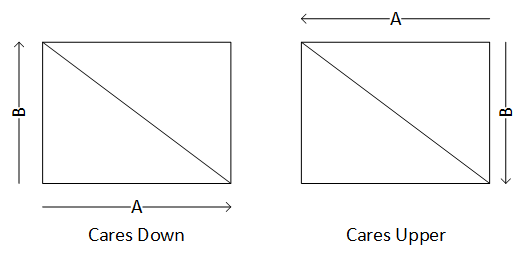
\includegraphics[width=0.4\textwidth]{caranormal}
	\caption{Pattern for the calculation of normal on the faces}
	\label{fig-normalcara}
\end{figure}

\begin{figure}[!h]
\centering
  	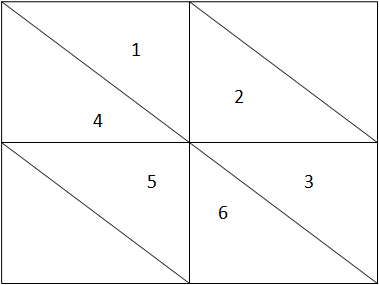
\includegraphics[width=0.2\textwidth]{vertexnormal}
	\caption{Pattern for calculation of normal at a vertex}
	\label{fig-normalvertex}
\end{figure}

Once the generation process has been completed, the application will generate a mesh that can be opened in any editor. As it can see in the figure \ref{fig-meshlab} it's open in software MeshLab.

\begin{figure}[!h]
\centering
  	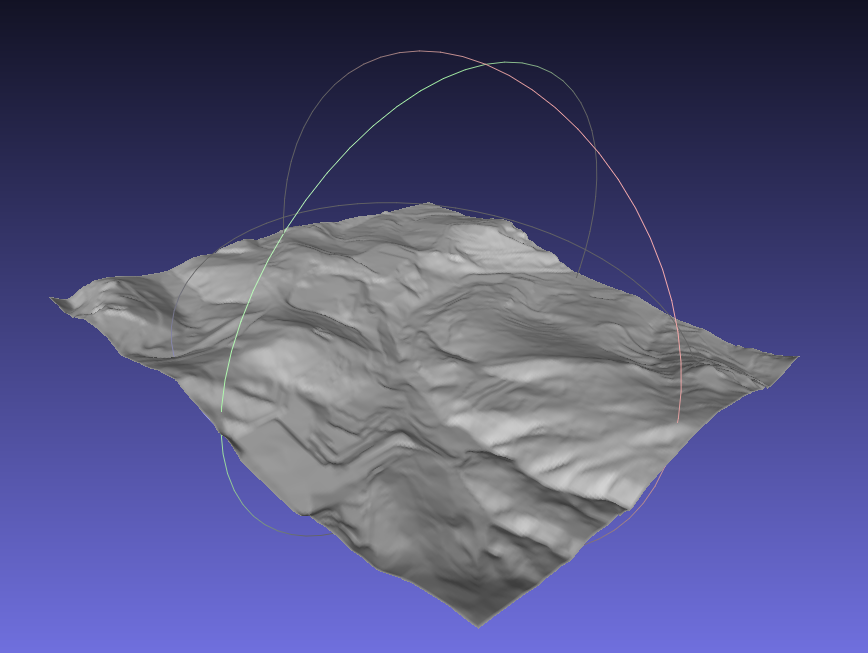
\includegraphics[width=0.35\textwidth]{mesh_example_meshlab}
	\caption{Terrain mesh visualized in software MeshLab}
	\label{fig-meshlab}
\end{figure}

\subsubsection{GEOJson associated at the terrain}

In order to can localize the terrain generated in other software that working with geospatial data or in the same simulator Unreal, it's decided to include in the generation a GEOJson that indicates the area which belongs the files generated. It's can see an example of this in the appendix \ref{appendix:geojson}.

\subsection{Time of generation}
In this section it's analyse the two versions implemented and can see the difference in time of generation. This is an important point for future implementations in which will wish implement a viewer in real time that loading new data according to the user moves for the world.
\\
On the figure \ref{fig-meshtime} can see the time spent from the version with loops for and the version implemented with NumPy, can see when realised the implementation using the library NumPy are reducing the time in 24x for a size of 500*500, this is due to the fact that NumPy is optimized for a parallelise the processing of data vectorial way.

\begin{figure}[!h]
\centering
  	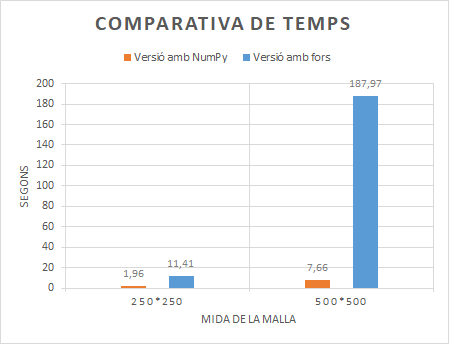
\includegraphics[width=0.4\textwidth]{meshtime}
	\caption{Graph with the time of generation of a mesh according to size}
	\label{fig-meshtime}
\end{figure}

\subsection{Quality}
\label{qualitat}
In this section is looking the form in which reduce the quality of terrain and can see the results obtained both qualitatively (visual difference) as quantitatively (size in bytes). In order to make this reduction are made skips of size "meshStep" set in the JSON configuration. It's made tests with powers of 2 (2, 4, 8, 16,...) on the own matrix of points and using the terrain of size 300x300 pixels.
\\
\\
As we can see in the figure \ref{fig-qualitatmegas} when reducing the amount of points, we reduce the size of the disk by exponentially, making the file load faster on the Unreal environment. As it's can see in the figure \ref{fig-qualityvisual} is visible the loss of quality taking as a reference the mountain in the background on this see the loss of definition at the top of the mountain. It's can consider visually that when it is configured ''meshStep'' on 1 or 2 the loss qualitative, not are appreciable, from 4 are starting to appreciate slightly, finally on the levels 8 and 16 its can see the most loss, where the top of the mountain can see simplified the apposite that it can see with the ''meshStep'' configured to 1 where can see a mountain range with a good definition.

\begin{figure}[!h]
\centering
  	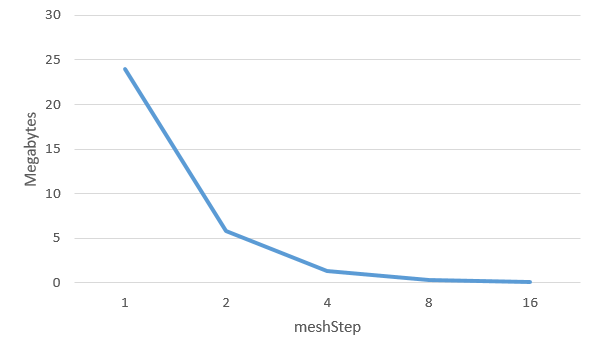
\includegraphics[width=0.4\textwidth]{qualitatmegas}
	\caption{Graphic with the size occupied on hard disk varying the ''meshStep'' parameter for a terrain of size 300x300.}
	\label{fig-qualitatmegas}
\end{figure}

\begin{figure}[!h]
\centering
  	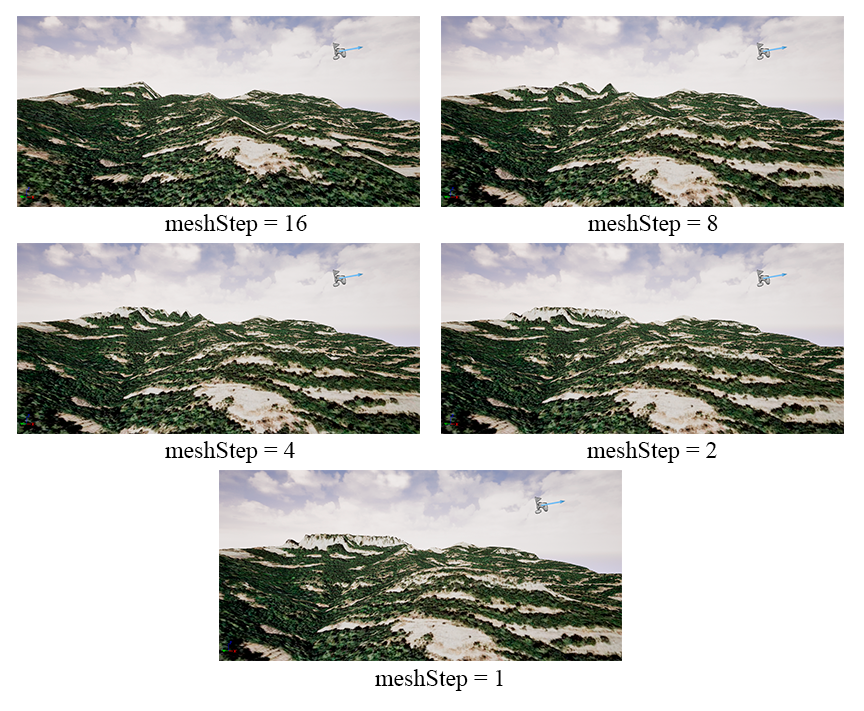
\includegraphics[width=0.5\textwidth]{quality/quality}
	\caption{Visual comparison of the effects produced by the level quality}
	\label{fig-qualityvisual}
\end{figure}

\newpage
\section{Module: Simulator}

In this section its explain the multiple parts of which is composed the module of simulation. The objective of this module is to make available a tool that allows simulate a travel with a generic vehicle above a terrain getting images from multiple cameras configured on board of the vehicle. A way to make this is providing the interface for control the vehicle with an external script sending commands with the RPC Protocol, in this case, it's implemented the server as can see in section \ref{rpcserver} and control it with a client implemented in a module as can you see in the section \ref{modulescript}.

\subsection{Visualization and control of the vehicle}

This part is based on providing the interface for moving a generic vehicle to the simulated world, this vehicle is configured with several cameras that are displayed on the screen and that can generate images of each one of them, in this way the possibility is added to view the same area in multiple perspectives. As an example, you can see an zenith view in the figure \ref{fig-montserratir}.

\begin{figure}[!h]
\centering
  	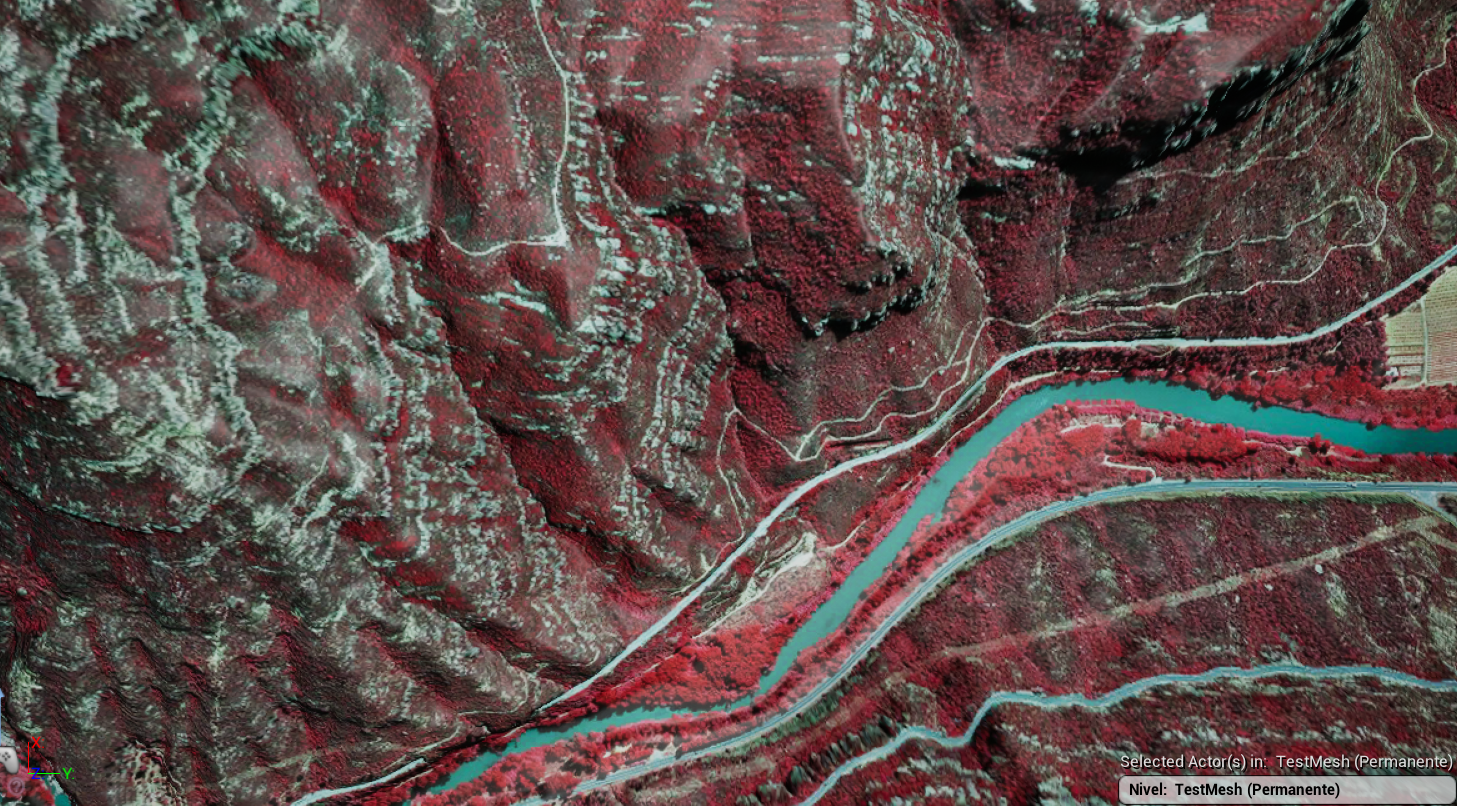
\includegraphics[width=0.5\textwidth]{cenitalviewir}
	\caption{Infrared view of Montserrat in zenith position}
	\label{fig-montserratir}
\end{figure}

\subsubsection{Remote control}
\label{rpcserver}

In the order to controller remotely the vehicle, it's implemented a communication using the RPC protocol (Remote Procedure Call) more concretely it's using the library Rpclib\cite{rpclib} for C++. This server is implemented in the Unreal module, the RPC server management is done through a class (AVehiclePawn) that can be inherited so that it offers basically the interface necessary to control a vehicle, specifically the following actions is implemented:

\begin{itemize}
\item Initialize/stop the RPC server: Initialize the server by pressing the Y cloth to the simulator of Unreal and stop it with the U key.
\item Change the position of the vehicle.
\item Change rotation of the vehicle or cameras (Implemented with LookAt).
\item Ask for images from one of the cameras to be generated.
\end{itemize}

The assignment of the functionalities is done in the function ''void BindFunctions(rpc::server* server)'' which receives the instance of the server, this function can be overridden to later be added to legacy classes with more functionality as can be seen in the annex \ ref {appendix: extendrpc}. By default the AVehiclePawn class allows us to call the following RPC functions:

\begin{itemize}
\item setLocation(double x, double y, double z): Enviem la localització en la qual volem que és situí el nostre vehicle.

\item setLookAt(double x, double y, double z): Enviem el vector amb la posició en el món que volem visualitzar, d'aquesta forma calcularem en quin punt del simulador es ha de mantenir la vista de la càmera.

\item setLocationAndLookAt(double x, double y, double z, double lx, double ly, double lz): Funció que crida d'un a les dues anteriors.

\item setCameraLookAt(int cameraId, double x, double y, double z): Funció que canvia la direcció en la que mira la càmera que l'indiquem.

\item getImage(int idCamera, std::string path): Ens permet indicar de quina càmera i on volem guardar la imatge.
\end{itemize}

\subsubsection{Visualització del cel}
Per tal d'implementar el cel hem utilitzat un modul natiu d'Unreal que ens permet generar una sphere en la que es renderitza un cel aquest cel té diversos paràmetres ajustables que ens permet determinar la posició del sol en aquell moment, el nivell de brillantor de les estrelles, la quantitat de núvols, etc. 
\\\\
Això dona la possibilitat de generar imatges sintètiques en diferents moments del dia amb diferents il·luminacions, el que permetrà generar datasets més complexos. D'altra banda això comportarà que haurem d'aplicar textures sense ombres per tal que aquestes siguin generades per al motor d'Unreal. Podem veure un exemple de diferents hores del dia a la figura \ref{fig-sky}.

\begin{figure}[!h]
\centering
  	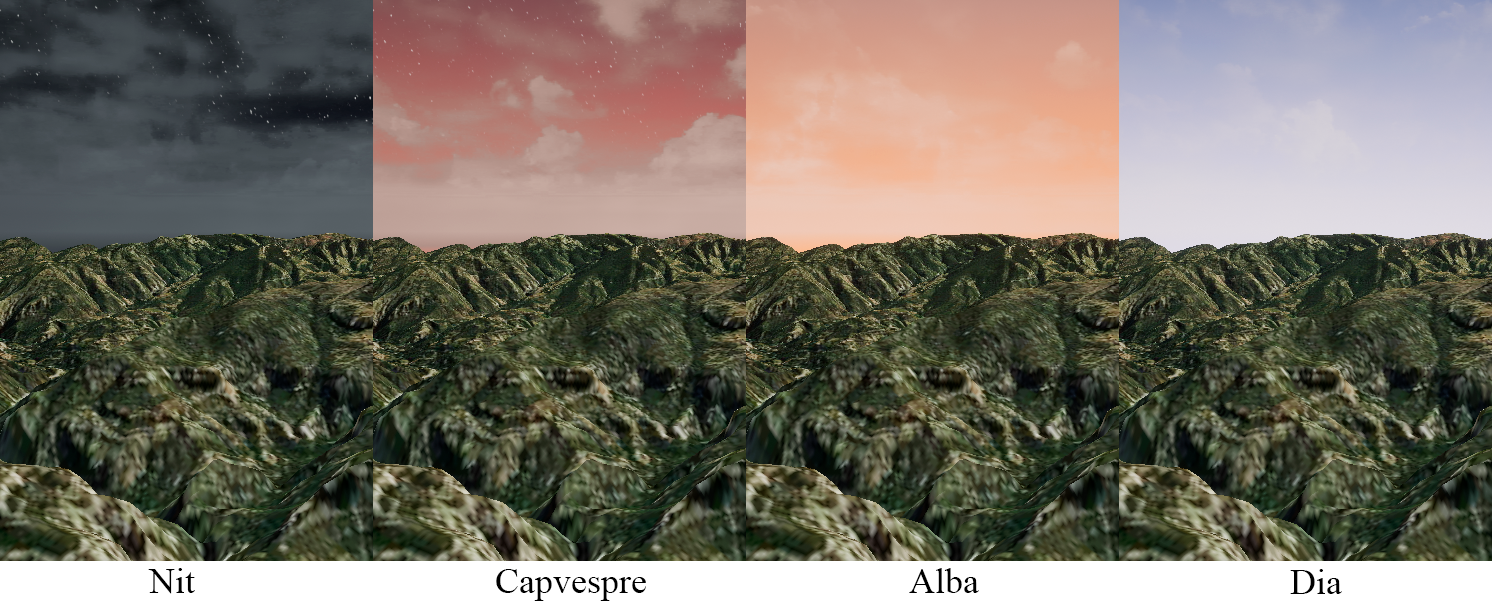
\includegraphics[width=0.48\textwidth]{sky/sky}
	\caption{Exemple de cels}
	\label{fig-sky}
\end{figure}

\subsection{Terreny}
El terreny és carregat mitjançant codi obtenint el fitxer .obj i processant aquest fitxer per tal de generar una malla en temps d'execució generant un UProceduralMesh\cite{uprocedural} d'Unreal, per tal de realitzar aquesta tasca es té en compte que Unreal treballa amb un sistema de coordenades invertit respecte al model UTM en el qual l'eix Y es troba invertit a conseqüència d'això es ha de realitzar la reflexió en l'eix Y els objectes fent la correspondència que pertoqui en cada moment entre el món real i el món simulat.
\\
\\
Aquesta malla és carregada al món i representada per la classe ''MapChunk'' al qual se li assignarà el material dinàmic que contindrà les textures carregades de les diferents visualitzacions que desitgem podent visualitzar qualsevol de les imatges que preparem en format imatge per al terreny com poden ser textures RGB, Infraroig, multi espectral, etc.

\subsection{Visualització del terreny}
En aquest apartat veurem els resultats obtinguts a partir de terrenys 3D generats pel mòdul GEOTool i l'aplicarem diverses visualitzacions de fonts com són textures o shaders obtinguts per diversos medis, en concret les vistes RGB i infraroig són obtingudes de l'Institut Cartogràfic de Catalunya, les dades multiespectrals les obtenim de l'explorador EO Browser\cite{eobrowser} i la informació de profunditat l'obtenim d'aplicar un shader a l'escena.
\\
\\
Com podem veure en la figura \ref{fig-bands} hem aplicat a un terreny corresponent a ''Sales de Pallars'' diferents bandes multiespectrals obtingudes pel satèl·lit Sentinel 2\cite{sentinel2}. Les tres primeres bandes B02, B03 i B04 corresponen a bandes de colors, la banda B05 correspon al canvi ràpid de reflectància que fa la vegetació en un rang proper a l'infraroig, la banda B08 obté informació NIR\cite{nir} i per últim veiem la banda B09 capaç de detectar vapors d'aigua.

D'aquesta forma amb aquestes bandes podem obtenir informació composta per diversos espectres que podem aplicar a diversos àmbits. En la figura \ref{fig-spectralindexes} es poden veure alguns exemples, entre ells podem veure índexs com són:

\begin{itemize}
\item 
{
	NVDI\cite{ndvi}: Basat en la combinació de les bandes (B08 - B04)/(B08 + B04), índex utilitzat per veure l'estat del conreu.
}
\item
{
	Moisture index\cite{moisture}: Basat en la combinació de les bandes (B8A - B11)/(B8A + B11), indica la proporció de precipitació que es necessita per tal de satisfer les necessitats de la vegetació.
}
\item
{
	NDWI\cite{ndwi}: Basat en la combinació de les bandes (B03 - B08)/(B03 + B08), índex que s'utilitza per determinar l'estrès hídric de la vegetació, saturació de la humitat en el terra o realitzar delimitacions de masses d'aigua com a llacs o embassaments.
}
\end{itemize} 

En l'última vista de la figura \ref{fig-spectralindexes} es pot veure la de profunditat o proximitat utilitzada per algoritmes de reconstrucció 3D amb monocular stereo, prevenció de col·lisions, algoritmes de multiview stereo, etc.

\begin{figure*}[!h]
\centering
  	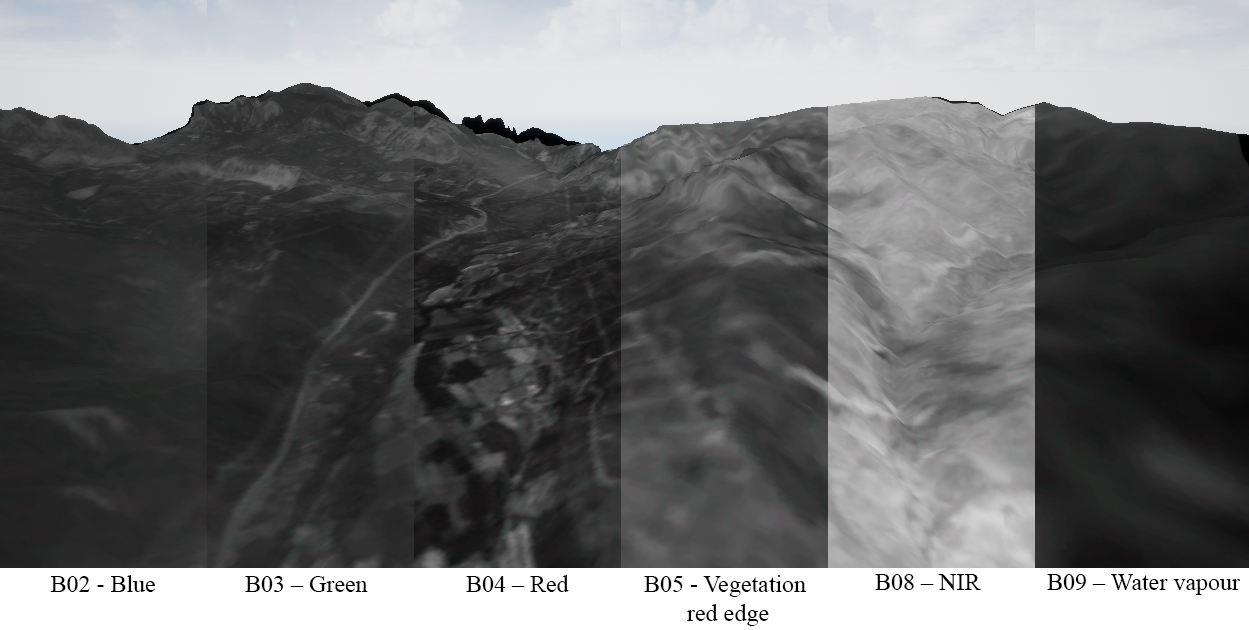
\includegraphics[width=1\textwidth]{multispectral/bands}
	\caption{Vista de Sales de Pallars en 6 bandes diferents}
	\label{fig-bands}
\end{figure*}

\begin{figure*}[!h]
\centering
  	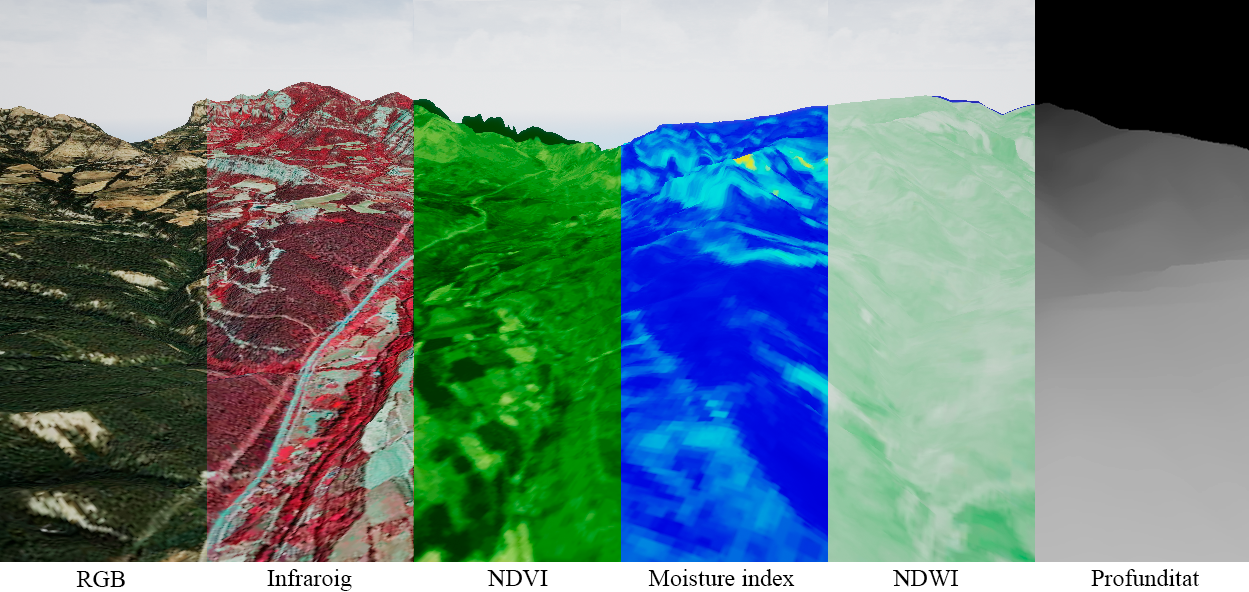
\includegraphics[width=1\textwidth]{multispectral/spectralindexes}
	\caption{Vista de Sales de Pallars en RGB, Infraroig, NDVI, Moisture, NDWI i profunditat}
	\label{fig-spectralindexes}
\end{figure*}

\subsection{Interacció amb el simulador}
Per tal d'interaccionar amb el simulador s'han definit les següents tecles:

\begin{itemize}
\item A,W,S,D: Per moure'ns en el simulador.
\item Q,E: Per rotar la vista.
\item Y: Inicia el servidor RPC.
\item U: Para el servidor RPC.
\item H: Mostra/oculta la visualització del vehicle.
\item K: Guarda en un fitxer la vista actual de la segona càmera.
\end{itemize}

\section{Mòdul d'Scripting}
\label{modulescript}
En aquest apartat explicarem i veurem els principals punts del mòdul d'scripting en el qual podrem gestionar el simulador de forma que podrem recrear viatges llegint fitxers de trajectòries, generar imatges, generar soroll a les trajectòries, etc.

\subsection{Trajectòries}
El mòdul d'scripting permet fer vols llegint trajectòries creades en el món real (adaptant-les al nostre format) o generades sintèticament d'aquesta forma podem recrear en el simulador la trajectòria feta anteriorment podent reproduir tants cops com vulguem aquesta, això ens permetrà fer diverses proves amb diferents visualitzacions del terreny. Per aquesta finalitat s'ha generat el fitxer que expliquem a la secció \ref{file-trajectories}.

\subsubsection{Fitxer de trajectòries}
\label{file-trajectories}
En aquest apartat explicarem com està formatjat el fitxer de trajectòries i el fitxer per posicionar la càmera. Els fitxers estaran en format CSV i seran llegits des de mòdul GEOControl per a indicar al simulador les posicions del vehicle i cap a quina posició del món mira tant el vehicle com les càmeres.

El fitxer que controla al vehicle està compost pels següents camps:

\begin{itemize}
\item Time: Temps en mil·lisegons d'ençà que comença el script.
\item x: Posició X en format UTM.
\item y: Posició Y en format UTM.
\item z: Posició Z en format UTM.
\item LookX: Posició X a la que mirem en format UTM.
\item LookY: Posició Y a la que mirem en format UTM.
\item LookZ: Posició Z a la que mirem en format UTM.
\end{itemize}

Per tal de controlar a on miran les cameras tindrem un altre fitxer composat per els camps:

\begin{itemize}
\item Time: Time en milisegons des de que comença el script.
\item cameraId: Id de la camera que volem modificar.
\item LookX: Posició X a la que mirem en format UTM.
\item LookY: Posició Y a la que mirem en format UTM.
\item LookZ: Posició Z a la que mirem en format UTM.
\item GetImage: Booleà de 0 o 1 en el que indiquem si volem generar una imatge d'aquesta càmera en aquell instant de temps.
\end{itemize}

Podem veure un exemple dels fitxers CSV a l'apèndix \ref{appendix:fitxerscsv} generats amb Excel.

\subsection{Simulació de soroll}
Ja que els vehicles tenen moviments inesperats a conseqüència de l'aire, l'asfalt entre d'altres s'ha implementat un generador de soroll aplicat a la trajectòria que volem reproduir d'aquesta forma podem generar imatges amb soroll i moviments inesperats. Aquest soroll s'ha implementat mitjançant un soroll gaussià en el qual utilitzem com a centre el punt al qual ens volem moure i una sigma petita (entre 0 i 1) que ens generarà un moviment lleuger.

\subsection{Generació de Datasets}
Un dels objectius d'aquest treball és la possibilitat de generar datasets d'imatges sintètiques amb dades generades per satèl·lits, per tal de poder generar datasets s'utilitza el camp GetImage vist a la secció \ref{file-trajectories} que ens generarà una imatge cada cop que trobi aquest camp.

En la figura \ref{fig-dataset} podem veure una petita mostra amb poques imatges d'un recorregut en el qual hem fixat que la càmera mires a un punt en concret que deixàvem enrere amb el transcurs del temps. 

\begin{figure}[!h]
\centering
  	\includegraphics[width=0.45\textwidth]{dataset/dataset}
	\caption{Conjunt d'imatges generades per GEOControl}
	\label{fig-dataset}
\end{figure}

\section{Conclusions}
En aquest projecte hem vist com hem pogut obtenir textures i mapes d'elevacions de fonts procedents de satèl·lits i convertir-les en informació 3D que pugui ser afegida a un motor gràfic com és Unreal Engine. S'ha tingut en compte aspectes com la velocitat en generar el model 3D on s'ha pogut veure com afecta llibreries com NumPy en el tractament de matrius accelerant aquest procés gràcies a la paral·lelització, s'ha pogut veure l'efecte que té quantitativament i qualitativament en les malles en reduir la quantitat de punts amb els quals es genera el model 3D necessari per a la renderització de models de grans dimensions.

Per la part del mòdul simulador hem pogut veure com podem visualitzar informació en un entorn 3D generat amb Unreal Engine. Es poden afegir càmeres a un vehicle simulat i veure des de diferents perspectives una mateixa informació per això s'ha creat un altre modulo que envia comandes al servidor RPC que s'ha implementat en Unreal Engine el qual pot moure, dir cap a on mira el vehicle, dir cap a on mira les càmeres i obtenir imatges d'aquestes càmeres.
S'han fet proves amb diverses visualitzacions provinents d'informació de satèl·lits com és el Sentinel 2 en el que s'ha pogut veure com és representa'n en el món simulat i quines utilitats té aquesta informació.

Per la part del mòdul d'scripting s'ha vist com es poden generar trajectòries reproduïbles en l'entorn simulat per tal de fer diversos viatges amb diferents informacions i extraure dades en forma de dataset. Aquestes trajectòries poden controlar diversos paràmetres del vehicle i càmeres indicant en quins punts es vol obtenir una imatge i de quina càmera. Per tal de simular el moviment a causa del vent o altres factors s'ha afegit un petit filtre com és la generació de soroll per tal de fer que se sacsegi el vehicle.


\section*{Agraïments}

\begin{thebibliography}{11}
\bibitem{agile}
Agile software development
\\ \url{https://en.wikipedia.org/wiki/Agile_software_development}
[19/02/2019]

\bibitem{kanban}
Kanban
\\ \url{https://www.iebschool.com/blog/metodologia-kanban-agile-scrum/} [19/02/2019]

\bibitem{trello}
Trello - \url{https://trello.com/} [19/02/2019]

\bibitem{airsim}
AirSim - \url{https://github.com/Microsoft/AirSim} [19/02/2019]

\bibitem{carla}
Carla SIMULATOR - \url{http://carla.org} [19/02/2019]

\bibitem{less}
LESS - \url{http://lessrt.org/} [11/04/2019]

\bibitem{dirsig}
Digital Imaging and Remote Sensing Image Generation - \url{http://dirsig.org/} [11/04/2019]

\bibitem{googleearth}
Google Earth Engine - \url{https://earthengine.google.com/} [20/05/2019]

\bibitem{unreal}
Unreal Engine - \url{https://www.unrealengine.com/en-US/what-is-unreal-engine-4} [09/03/2019]

\bibitem{ogc}
Open Geospatial Consortium (OGC) -  \url{http://www.opengeospatial.org/} [08/04/2019]

\bibitem{wms}
Web Map Service (WMS) -  \url{https://www.opengeospatial.org/standards/wms} [08/04/2019]

\bibitem{wcs}
Web Coverage Service (WCS) -  \url{https://www.opengeospatial.org/standards/wcs} [08/04/2019]

\bibitem{icgc}
Institut Cartogràfic i Geològic de Catalunya (ICGC) - \url{http://www.icgc.cat/ca/} [08/04/2019]

\bibitem{wavefrontobj}
Wavefront .obj file - \url{https://en.wikipedia.org/wiki/Wavefront_.obj_file} [09/04/2019]

\bibitem{rpclib}
RPC Lib - Modern mgspack-rpc for C++ - \url{http://rpclib.net/} [10/04/2019]

\bibitem{uprocedural}
Procedural Mesh Component - \url{https://wiki.unrealengine.com/Procedural_Mesh_Component_in_C%2B%2B:Getting_Started} [21/05/2019]

\bibitem{eobrowser}
EO Browser - \url{https://apps.sentinel-hub.com/eo-browser/} [25/05/2019]

\bibitem{sentinel2}
Sentinel 2 - \url{https://www.esa.int/esl/ESA_in_your_country/Spain/SENTINEL_2} [25/05/2019]

\bibitem{nir}
Tecnología NIR, sus Usos y Aplicaciones - \url{https://www.engormix.com/balanceados/articulos/tecnologia-nir-sus-usos-t32534.htm} [25/05/2019]

\bibitem{ndvi}
El NDVI o Índice de vegetación de diferencia normalizada - \url{https://geoinnova.org/blog-territorio/ndvi-indice-vegetacion/} [25/05/2019]

\bibitem{moisture}
Moisture index - \url{http://glossary.ametsoc.org/wiki/Moisture_index} [25/05/2019]

\bibitem{ndwi}
Cálculo del índice NDWI - \url{http://www.gisandbeers.com/calculo-del-indice-ndwi-diferencial-de-agua-normalizado/} [25/05/2019]

\end{thebibliography}

\appendix
\section*{Apèndix}

\setcounter{section}{1}

\subsection{JSON d'exemple per la configuració de GEOTool}
\label{appendix:geotoolconfig}
\lstinputlisting{geotoolconfig.json}

\subsection{Codi per la generació d'una malla 3D a partir d'un fitxer d'altures}
\label{appendix:generateobj}
\lstinputlisting[language=Python]{generateobj.py}

\subsection{GEOJson d'exemple}
\label{appendix:geojson}
\lstinputlisting{geojson.json}

\subsection{Codi d'exemple per estendre la funcionalitat RPC}
\label{appendix:extendrpc}

\lstset{language=C} 
\begin{lstlisting}
.h:
	virtual void BindFunctions(rpc::server* server) override;
	
.cpp:
void MyClass::BindFunctions(rpc::server* server)
{
	Super::BindFunctions(server);

	server->bind("nameOfFunction", [context_params](Variables...) {
		//MyCode
	});
}

\end{lstlisting}

\subsection{Fitxers CSV d'exemple per controlar el vehicle i les càmeres}
\label{appendix:fitxerscsv}

\begin{figure}[!h]
\centering
  	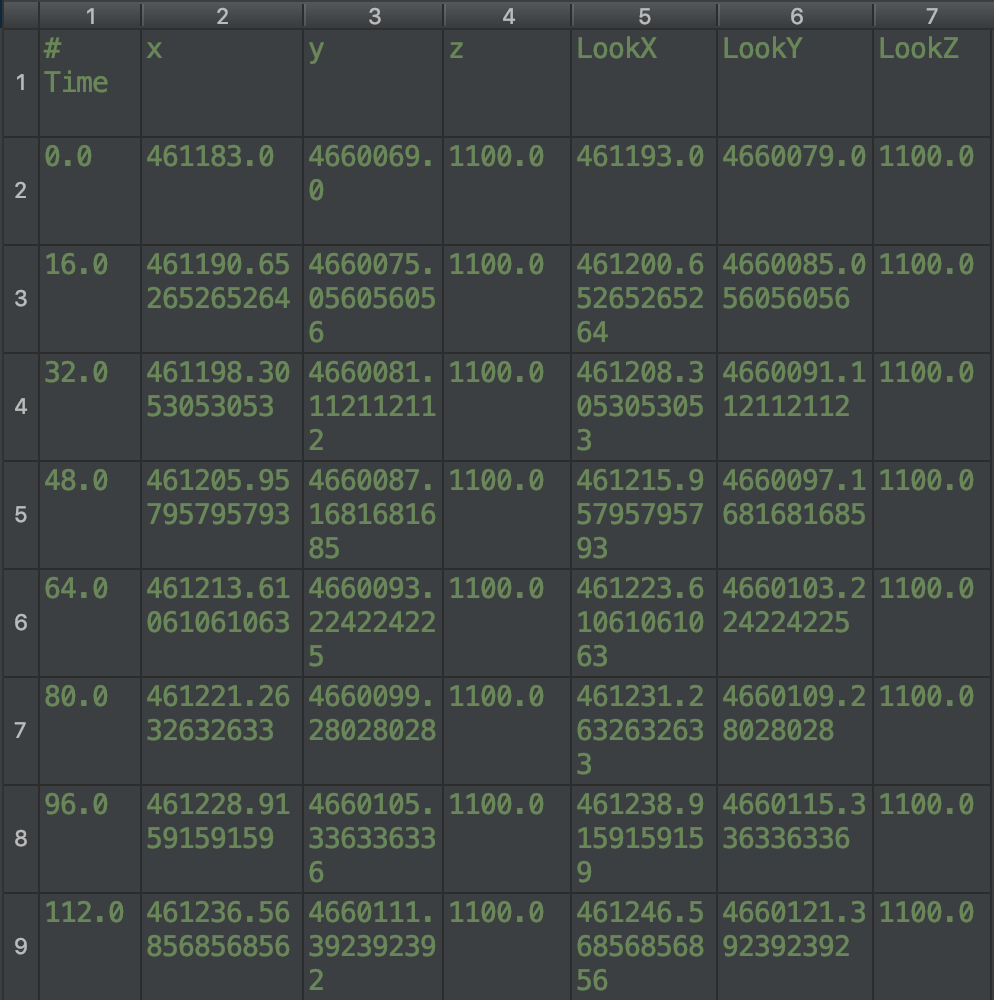
\includegraphics[width=0.45\textwidth]{fitxervehicle}
	\captionsetup{labelformat=empty}
	\caption{Fitxer CSV per controlar el vehicle}
	\label{fig-fitxervehicle}
\end{figure}


\begin{figure}[!h]
\centering
  	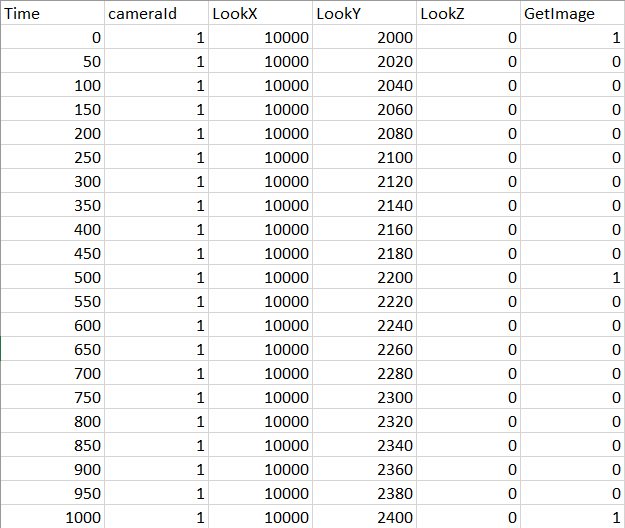
\includegraphics[width=0.45\textwidth]{fitxercameres}
  	\captionsetup{labelformat=empty}
	\caption{Fitxer CSV per controlar les càmeres}
	\label{fig-fitxercameres}
\end{figure}


\end{document}

